\chapter{Creation of the Artifact}
\label{creation_of_the_artifact}

\section{Initial Goals}

As this project was first and foremost a project, designed to interactively explore the problemspace from the perspective of the \ac{HPC} community, 
all the while being contained by business requirements and time constraints, the initial goals of this project were very broad and open ended. 
At first the initial goal was simply to create a \ac{PoC} of a realistic workflow engine using the "Arkouda" project,
in order to present the Customer with a easily graspable example of its capabilities.

In the first iteration of the project a preselector of possible Workflow management tools was presented from the business side,
with the option to increase the scope if the presented tools were not sufficient.

Therefore the goals of the first iteration of this project was twofold, first to determine which, if any, of the presented tools were suitable for the task at hand,
and to determine what would make an adequate \ac{PoC} for the customer.

\section{Selection of Workflow Management Tools}

As described in the previous section, the first iteration of this project was to determine which, if any, of the presented tools were suitable for the task at hand.
The initial choice of tools was:

\begin{itemize}
    \item \textbf{Pachyderm:} A \ac{k8s} based Workflow manager, written in go which was recently aquired by \ac{HPE}.
    \item \textbf{Argo:} A \ac{k8s} based Workflow manager , written in go, which is a \ac{CNCF} project.
    \item \textbf{\ac{CLASP}:}  An in-house developed workflow manager, written in Java, utilizing Serverlet to execute workflows\footcite{sayersCloudApplicationServices2015}.
    \item \textbf{Snaplogic:} A commercial workflow manager,
\end{itemize}

But given that it was possible to select projects outside of the initial selection, the following projects also need to be considered:


\begin{itemize}
    \item \textbf{Airflow:} A Python-based workflow manager under the \ac{CNCF} umbrella, known for its easy-to-use interface and extensibility.
    \item \textbf{Kubeflow:} A \ac{k8s}-native platform for deploying, monitoring, and running ML workflows and experiments, also a \ac{CNCF} project, streamlining \ac{ML} operations alongside other Kubernetes resources.
    \item \textbf{Knative:} An open-source ac{k8s}-based platform to build, deploy, and manage modern serverless workloads, simplifying the process of building cloud-native applications.
    \item \textbf{Luigi:} An open-source Python module created by Spotify to build complex pipelines of batch jobs, handling dependency resolution, workflow management, and visualization seamlessly.
    \item \textbf{\ac{CWL}:} An open-standard for describing analysis workflows and tools in a way that makes them portable and scalable across a variety of software and hardware environments, from workstations to cluster, cloud, and high-performance computing environments.
\end{itemize}
    
% ADD where this selection was taken from!!

\subsubsection{Selection Criteria}

Due to this extensive list of diverse tools, a set of criteria was established to determine which tool would be the most suitable for the task at hand.
% How should i justify the selection criteria??

\begin{itemize}
    \item \textbf{Ease of use:} 
    \item \textbf{Extensibility:}
    \item \textbf{Community and Support:}
    \item \textbf{Maturity:}
    \item \textbf{Integration with \ac{HPC} systems:}
    \item \textbf{Strategic alignment with \ac{HPE}:}
    \item \textbf{License:}
    \item \textbf{Cost:}
\end{itemize}

\newpage

\section{Design of the Artifact}





\begin{figure}[htb]
    \centering
    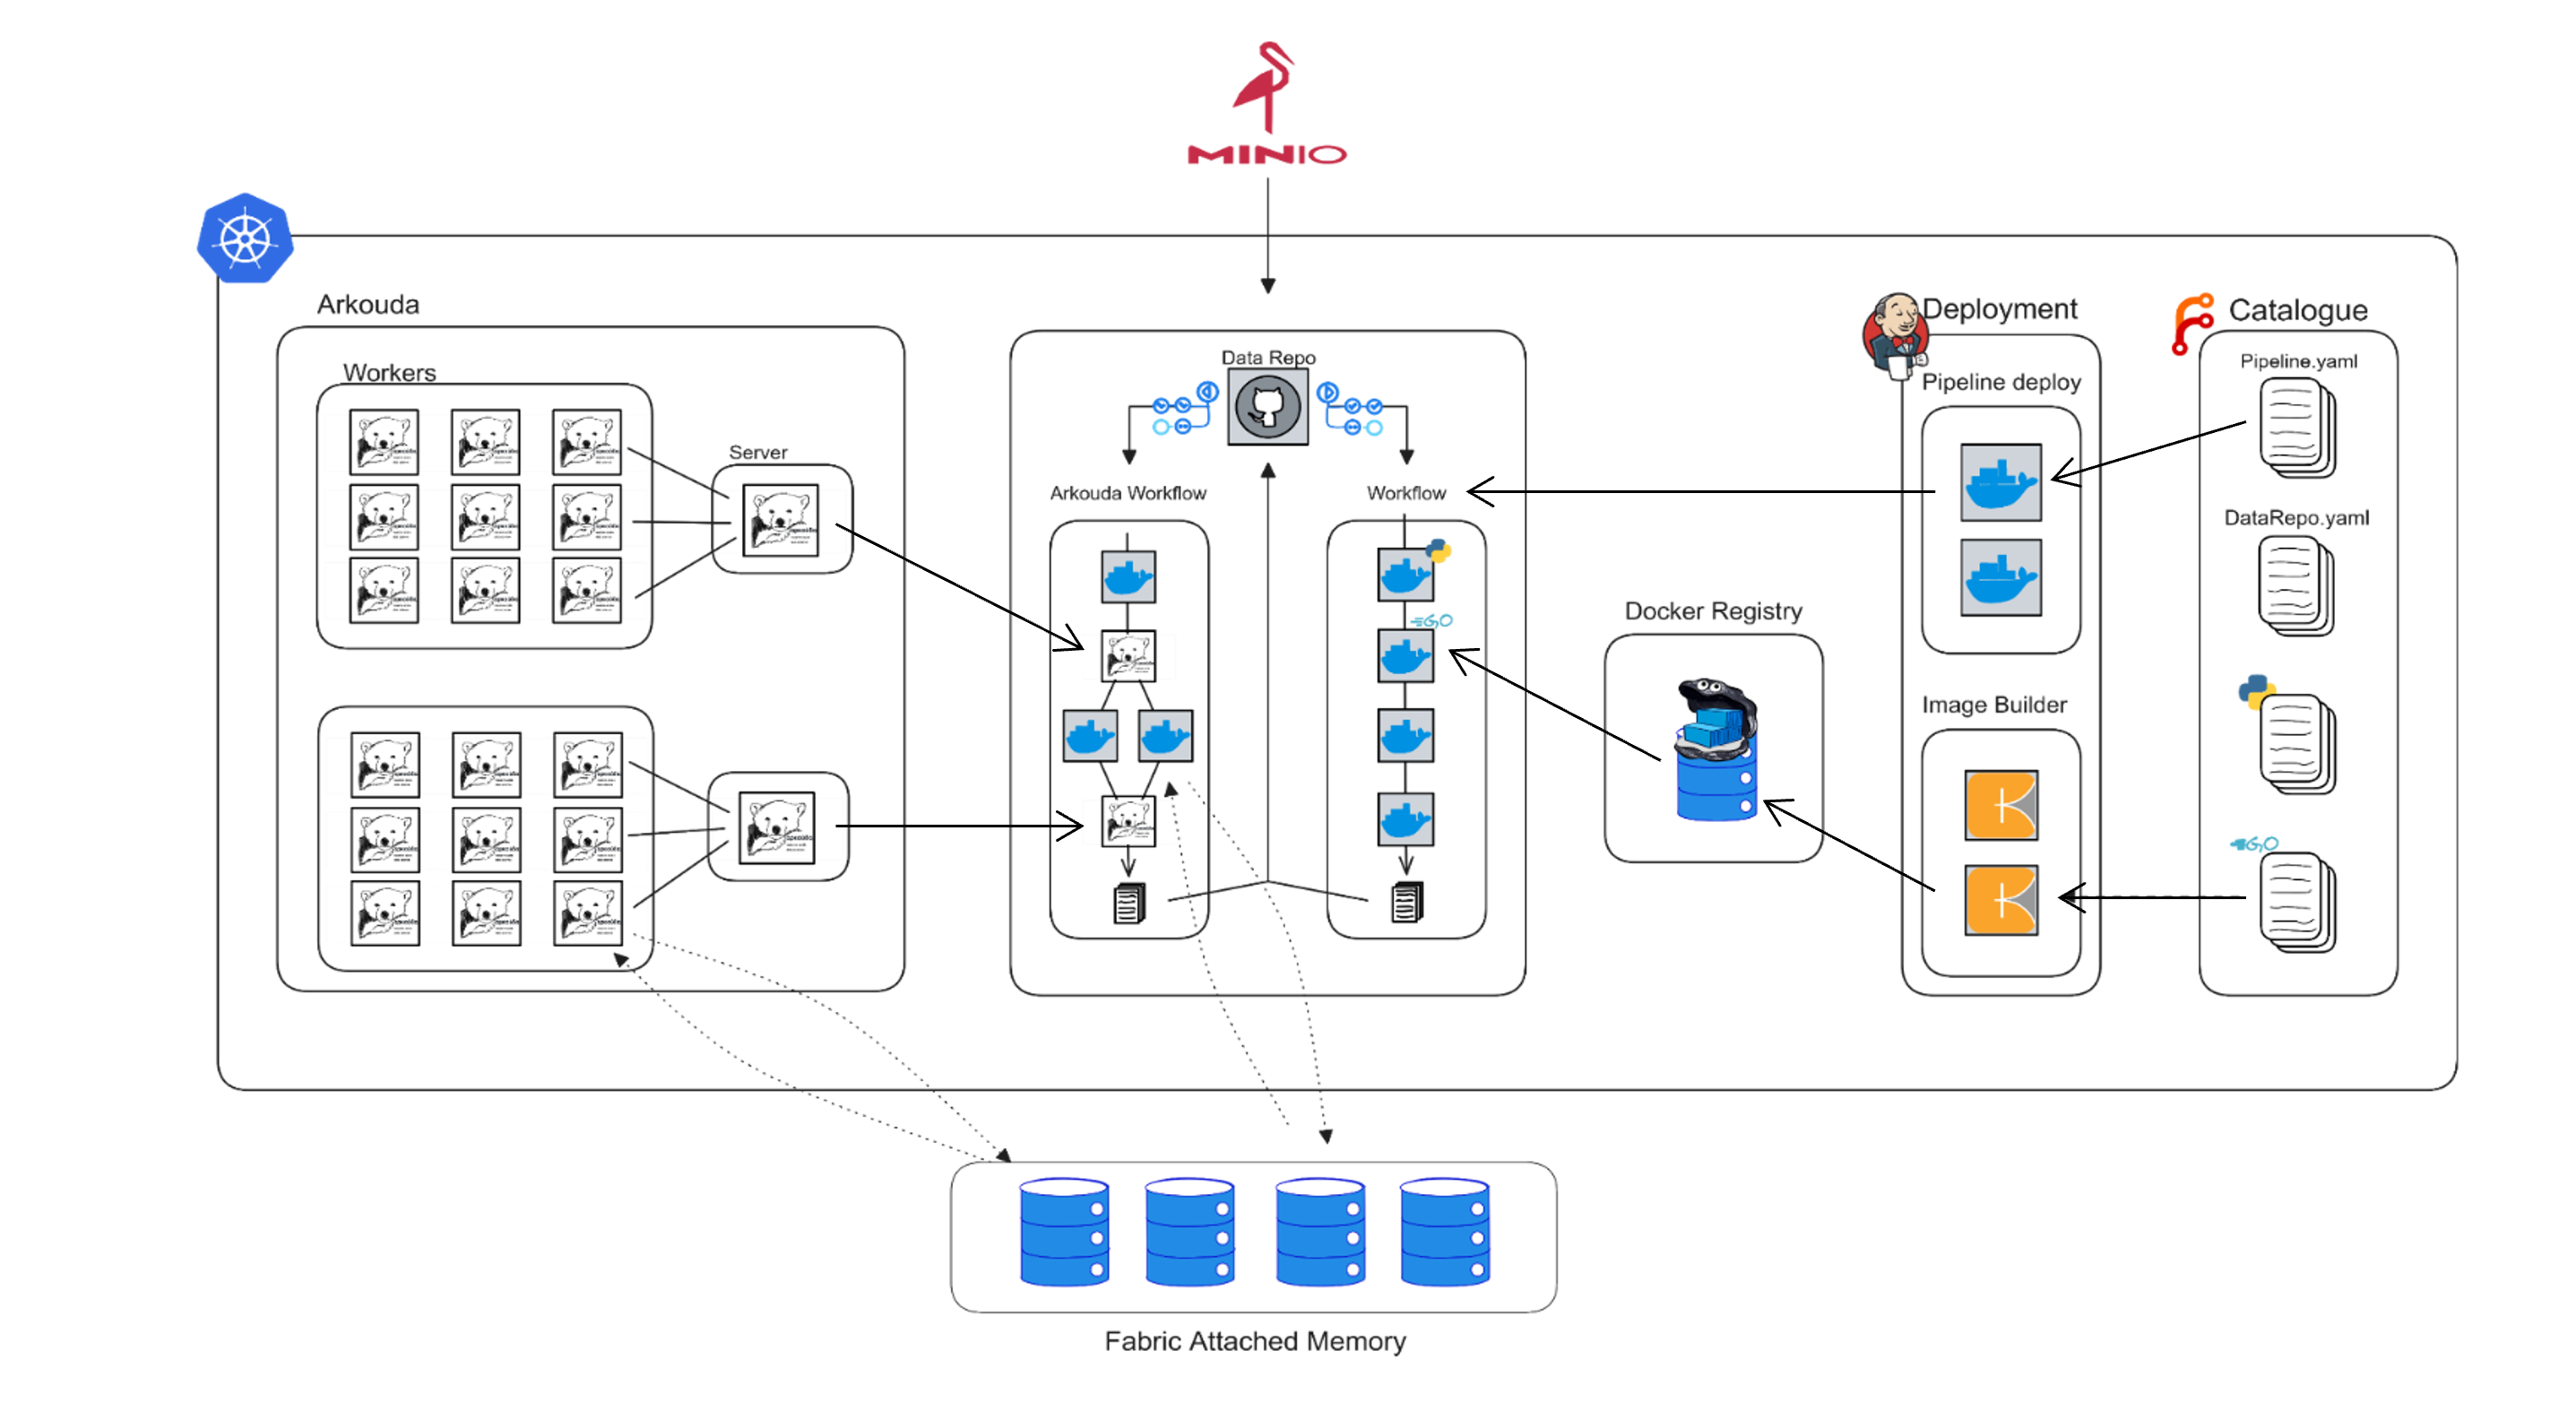
\includegraphics[width=16cm]{graphics/pachykouda.png}
    \caption[pachykouda high level diagramm]{Pachykouda high level infrastructure diagramm \footcite{eckerthHASPHPCApplications}}
    \label{abb:Logo2cmBreit}
\end{figure}


\newpage


\section{Implementation of the Artifact}



\newpage


\section{Evaluation of the Artifact}

\newpage
